% This file was automatically generated by flatten.py
% Source: supplement_main.tex
% Do not edit this file directly — edit the source files instead.
% ---------------------------------------------------------------

% supplement_main.tex
% Supplementary Material for:
% Solis-Lemus et al. | PLOS Computational Biology | PCOMPBIOL-D-25-02375
%
% Compile: ./rerunpdf.sh supplement_main
% Final:   ./rerunpdf.sh -f supplement_main
% -------------------------------------------------------------------------

\documentclass[10pt,letterpaper]{article}

\usepackage[top=1in,left=1in,right=1in,bottom=1in]{geometry}
\usepackage{cite}

% -------------------------------------------------------------------------
% SHARED PACKAGES AND MACROS
% -------------------------------------------------------------------------

% --- begin input: preamble_shared ---
% preamble_shared.tex
% Shared packages and macros for plos_latex_template.tex and supplement_main.tex
% DO NOT add layout/geometry/header packages here — those are file-specific.
% -------------------------------------------------------------------------

% Core math
\usepackage{amsmath,amssymb}

% Additional characters
\usepackage{textcomp,marvosym}

\usepackage[final,commentmarkup=footnote]{changes}  % use mode draft to show changes
\definechangesauthor[name={Reviewer 1}, color=blue]{R1}
\definechangesauthor[name={Reviewer 2}, color=orange]{R2}
\definechangesauthor[name={Reviewer 3}, color=teal]{R3}
\definechangesauthor[name={Multiple Reviewers}, color=magenta]{MR}
\definechangesauthor[name={Editor}, color=brown]{ED}
\definechangesauthor[name={PLOS Final Submission}, color=violet]{PLOS}


% Hyperlinks (nameref required for SI cross-references)
\usepackage{nameref,hyperref}

% Color (table shading)
\usepackage[table]{xcolor}

% Table utilities
\usepackage{array}
\usepackage{booktabs}

% Thick rule helpers (used in main manuscript tables)
\newcolumntype{+}{!{\vrule width 2pt}}
\newlength\savedwidth
\newcommand\thickcline[1]{%
  \noalign{\global\savedwidth\arrayrulewidth\global\arrayrulewidth 2pt}%
  \cline{#1}%
  \noalign{\vskip\arrayrulewidth}%
  \noalign{\global\arrayrulewidth\savedwidth}%
}
\newcommand\thickhline{%
  \noalign{\global\savedwidth\arrayrulewidth\global\arrayrulewidth 2pt}%
  \hline
  \noalign{\global\arrayrulewidth\savedwidth}%
}

% -------------------------------------------------------------------------
% SHARED MACROS
% -------------------------------------------------------------------------

% Simulation output symbols
\newcommand{\TAT}[1]{\ensuremath{\mathrm{TAT}_{#1}}}
\newcommand{\VOL}[1]{\ensuremath{\mathrm{Vol}_{#1}}}
\newcommand{\deltaVol}[1]{\ensuremath{\Delta \mathrm{Vol}_{#1}}}
\newcommand{\deltaVolNorm}[1]{\ensuremath{\mathcal{V}_{#1}}}

% Anatomical abbreviations
\newcommand{\LV}{LV}
\newcommand{\RV}{RV}
\newcommand{\LA}{LA}
\newcommand{\RA}{RA}
\newcommand{\SAN}{SAN}
\newcommand{\UKBB}{UKBB}

% Clinical group abbreviations
\newcommand{\Ctl}{$C$}
\newcommand{\HF}{$HF$}
\newcommand{\HFN}{$HF_N$}
\newcommand{\HFW}{$HF_W$}
% --- end input:   preamble_shared ---

\usepackage{lastpage,fancyhdr,graphicx}
\usepackage{xr}
\externaldocument{manuscript}
\externaldocument{sections/methods}

% -------------------------------------------------------------------------
% SUPPLEMENT-SPECIFIC LAYOUT
% -------------------------------------------------------------------------

% S-numbered figures and tables
\setcounter{figure}{0}
\renewcommand{\thefigure}{S\arabic{figure}}
\setcounter{table}{0}
\renewcommand{\thetable}{S\arabic{table}}

% Sections as S1, S2... (optional — comment out if you prefer plain numbering)
\renewcommand{\thesection}{S\arabic{section}}

% Captions
\usepackage[aboveskip=1pt,labelfont=bf,labelsep=period,
            justification=raggedright,singlelinecheck=off]{caption}
\renewcommand{\figurename}{Fig}
\renewcommand{\tablename}{Table}

% Header/footer
\usepackage{lastpage,fancyhdr}
\pagestyle{fancy}
\fancyhf{}
\rfoot{\thepage/\pageref{LastPage}}
\lfoot{Solis-Lemus et al. --- Supplementary Material}
\renewcommand{\headrulewidth}{0pt}
\renewcommand{\footrule}{\hrule height 1pt \vspace{2mm}}

% Line numbers (comment out if not wanted in supplement)
\usepackage[right]{lineno}

% Ligatures
\usepackage[nopatch=eqnum]{microtype}
\DisableLigatures[f]{encoding = *, family = * }

% Bibliography
\bibliographystyle{plos2025}
\makeatletter
\renewcommand{\@biblabel}[1]{\quad#1.}
\makeatother

% Text layout
\raggedright
\setlength{\parindent}{0.5cm}

% =========================================================================
\begin{document}

\begin{center}
    {\Large\textbf{Supporting Information}}\\[6pt]
    {\normalsize Solis-Lemus et al. | \textit{PLOS Computational Biology} |
    PCOMPBIOL-D-25-02375}
\end{center}

\bigskip
\linenumbers

% -------------------------------------------------------------------------
% S1 FIGURE: Whole-heart cohort reconstructions (moved from main per reviewer)
% -------------------------------------------------------------------------

% --- begin input: sections/supp/s_fig1_hearts ---
\subsection*{S1 Fig. Whole-heart cohort reconstructions.}
\begin{figure}[hbpt]
    \centering
    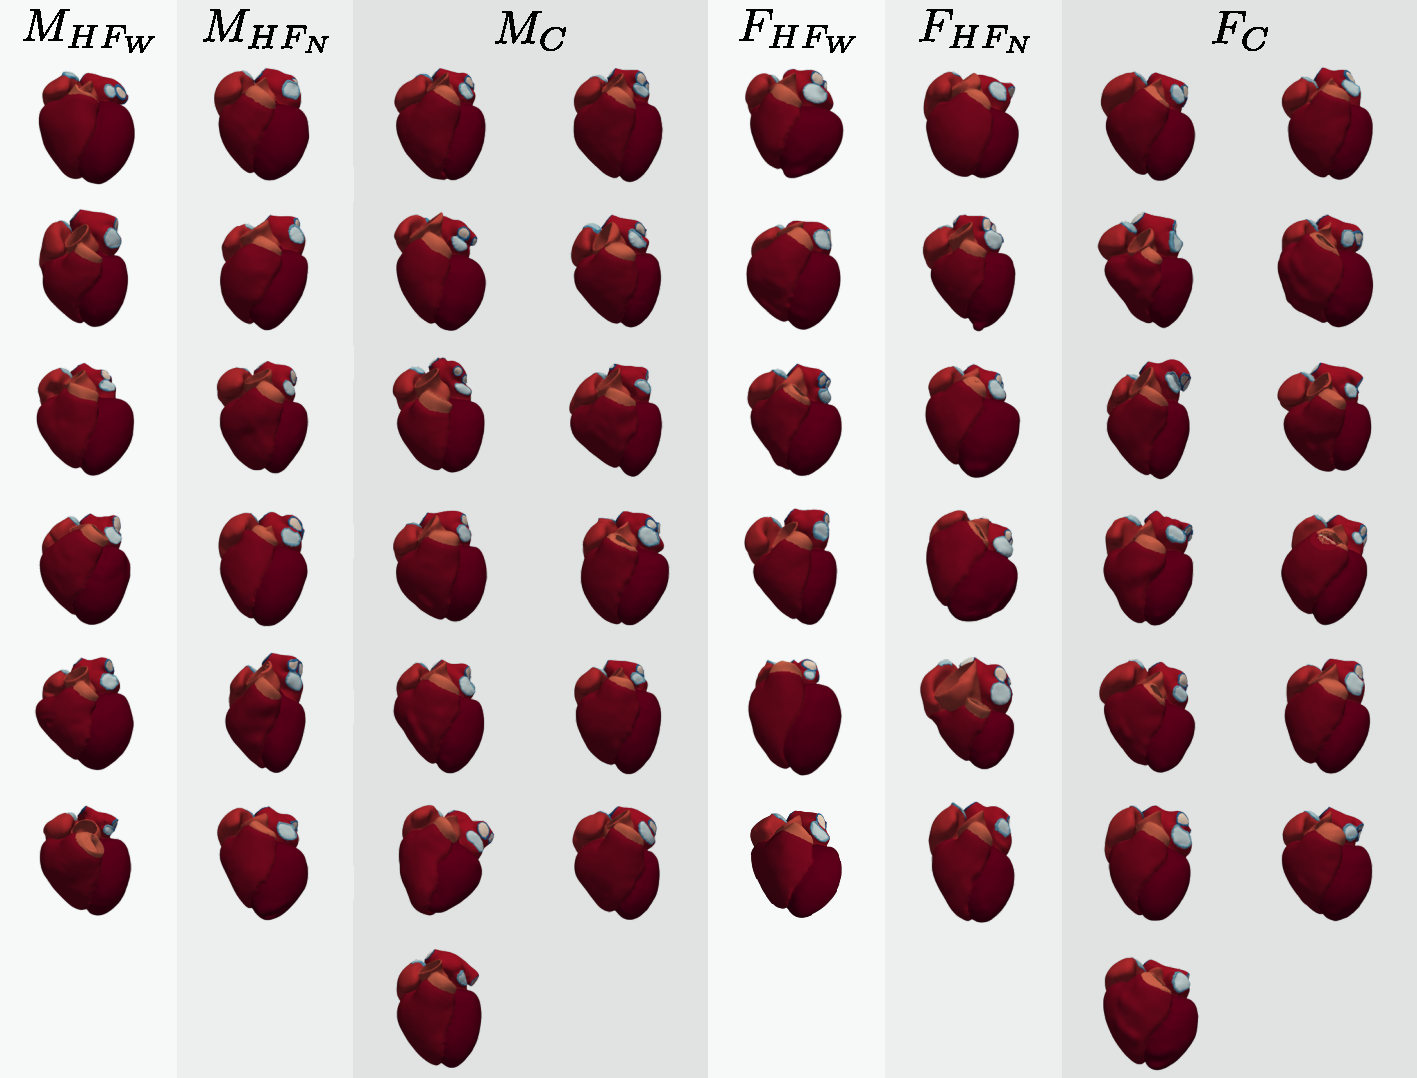
\includegraphics[width=\linewidth]{S1_Fig}
    \caption[Three-dimensional whole-heart reconstructions from the virtual cohort]{
        \textbf{Three-dimensional whole-heart reconstructions from the virtual cohort, grouped }
        and labelled by sex and condition. Each colour corresponds to a different structure in the mesh.
        Each model was derived from a patient's CT scan and includes fibre orientations,
        illustrating anatomical variability across sex and heart-failure subtypes.
        Abbreviations: $M_{HF_N}$: Male, HF narrow-QRS; $M_{HF_W}$: Male, HF wide-QRS; $M_C$: Male, Control;
        $F_{HF_N}$: Female, HF narrow-QRS; $F_{HF_W}$: Female, HF wide-QRS; $F_C$: Female, Control.
    }
    \label{fig:s1-hearts}
\end{figure}

% --- end input:   sections/supp/s_fig1_hearts ---

\newpage
% -------------------------------------------------------------------------
% S2 FIGURE: TAT-QRS Correlation
% -------------------------------------------------------------------------

% --- begin input: sections/supp/s_fig2_tat_qrs ---
\subsection*{S2 Fig. TAT-QRS correlation, stratified by condition.}
\begin{figure}[htbp]
    \centering
    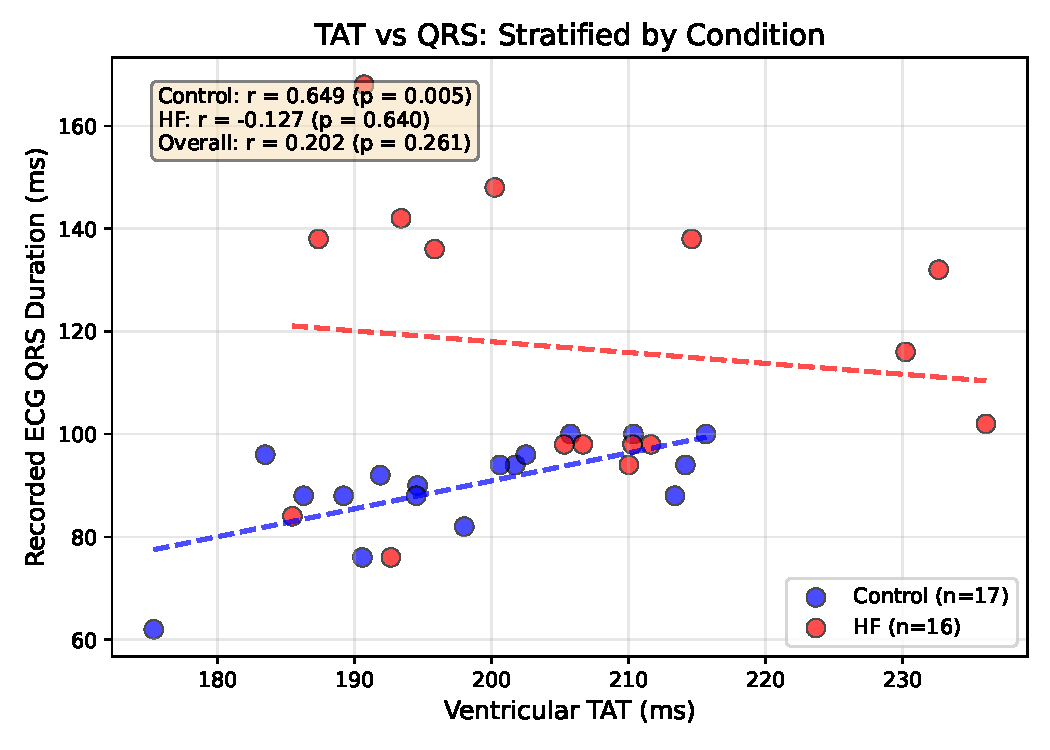
\includegraphics[width=\textwidth]{S2_Fig}
    \caption{
        \textbf{Correlation between simulated ventricular total activation time
        (\TAT{V}) and recorded ECG QRS duration, stratified by condition.}
        In \Ctl{} hearts (blue, $n=17$), \TAT{V} showed a strong positive
        correlation with QRS duration (Pearson $r = 0.649$, $p = 0.005$),
        indicating that anatomical variability alone can predict conduction time
        in healthy myocardium when using uniform electrophysiological parameters.
        In \HF{} patients (red, $n=16$), no correlation was observed
        ($r = -0.127$, $p = 0.64$), reflecting that pathological conduction
        delays (fibrosis, scar, conduction blocks) are not captured by anatomy
        alone and would require patient-specific tissue property calibration.
    }
    \label{fig:s2-tat-qrs}
\end{figure}

% --- end input:   sections/supp/s_fig2_tat_qrs ---



% -------------------------------------------------------------------------
% S1 TABLE: Geometric Characteristics
% -------------------------------------------------------------------------

% --- begin input: sections/supp/s_tab1_geometric ---
\subsection*{S1 Table. Geometric characteristics by sex and heart failure status.}
\begin{table}[htbp]
\centering
\caption{
    \textbf{Geometric characteristics stratified by sex and heart failure status.}
    Mean $\pm$ SD reported for age (years), chamber volumes (mL), and myocardial
    wall volume (cm$^3$). \HF{} patients showed increased chamber volumes across
    all chambers, particularly pronounced in males. Myocardial wall volume scaled
    with anatomical size, reflecting whole-heart structural differences across groups.
}
\begin{tabular}{lccccccr}
\toprule
\textbf{Group} & $n$ & \textbf{Age (yr)} &
    $\VOL{\LV}$ \textbf{(mL)} & $\VOL{\RV}$ \textbf{(mL)} &
    $\VOL{\LA}$ \textbf{(mL)} & $\VOL{\RA}$ \textbf{(mL)} &
    \textbf{Wall Vol. (cm$^3$)} \\
\midrule
Male \Ctl   & 13 & $47.2 \pm 12.0$ & $179.6 \pm 36.3$ & $188.7 \pm 25.7$
            & $93.9 \pm 27.9$  & $100.7 \pm 16.9$ & $319.0 \pm 43.7$ \\
Male \HF    & 12 & $60.1 \pm 16.1$ & $289.1 \pm 88.1$ & $227.6 \pm 60.2$
            & $140.5 \pm 58.9$ & $138.2 \pm 67.7$ & $396.0 \pm 75.2$ \\
Female \Ctl & 13 & $49.5 \pm  9.8$ & $139.7 \pm 32.2$ & $139.7 \pm 34.8$
            & $79.6 \pm 19.4$  & $86.3 \pm 32.3$  & $262.6 \pm 36.5$ \\
Female \HF  & 12 & $60.1 \pm  9.0$ & $183.0 \pm 60.0$ & $136.7 \pm 30.8$
            & $104.9 \pm 57.4$ & $100.0 \pm 47.3$ & $297.3 \pm 50.0$ \\
\bottomrule
\end{tabular}
\label{tab:s1-geometric-characteristics}
\end{table}
% --- end input:   sections/supp/s_tab1_geometric ---


% -------------------------------------------------------------------------
% S3 FIGURE: Correlation Heatmap
% -------------------------------------------------------------------------

% --- begin input: sections/supp/s_fig3_correlation_heatmap ---
\subsection*{S3 Fig. Geometry-output correlation matrix.}
\begin{figure}[htbp]
    \centering
    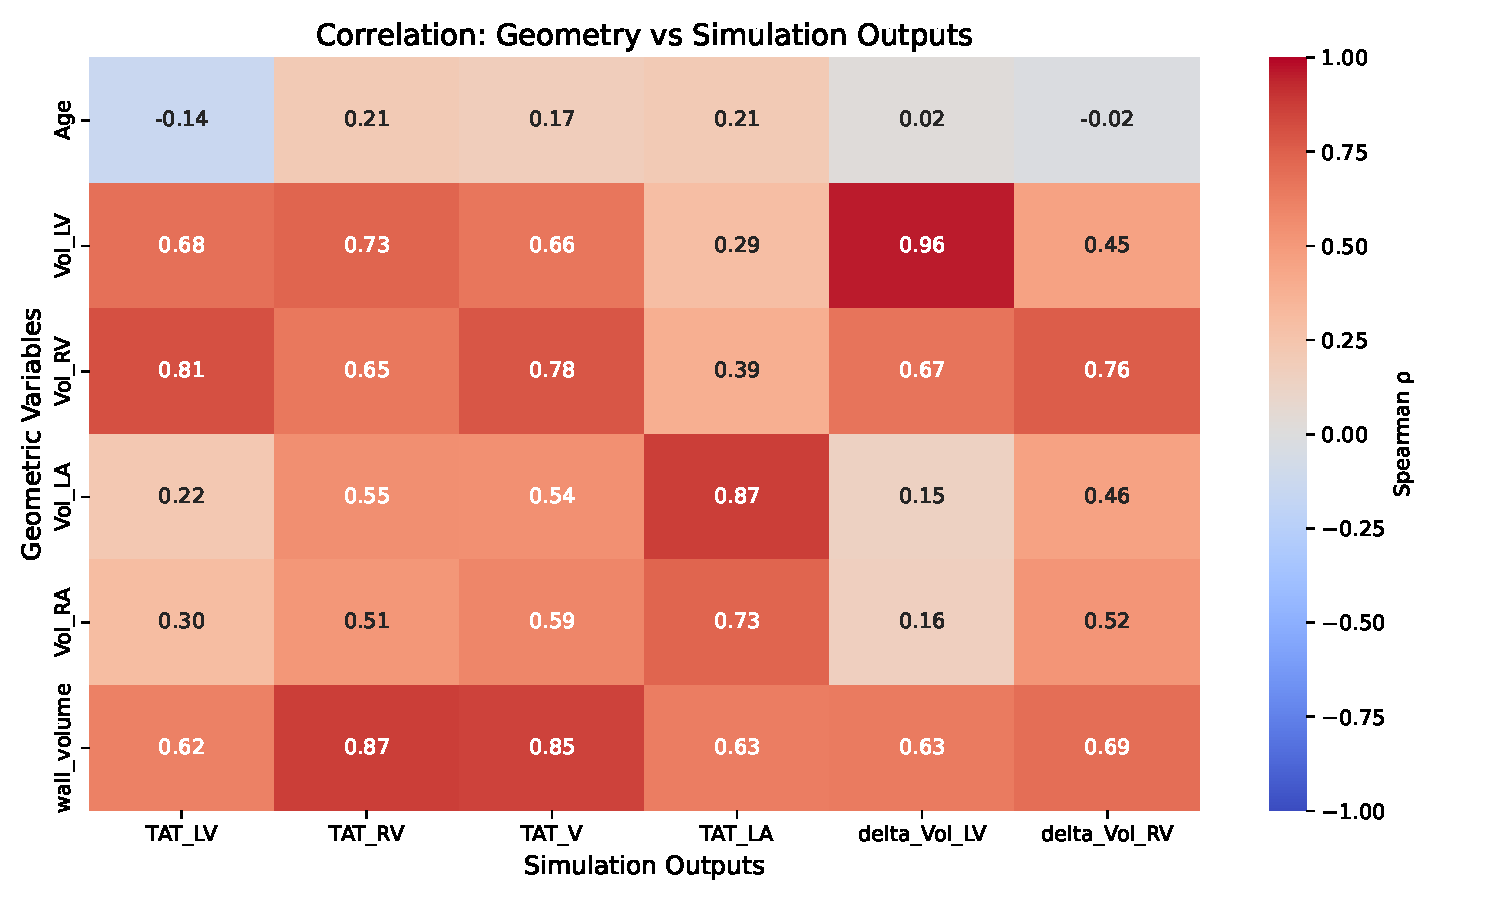
\includegraphics[width=\textwidth]{S3_Fig}
    \caption{
        \textbf{Correlation matrix between geometric variables and simulation outputs.}
        Spearman correlation coefficients ($\rho$) shown for relationships between
        geometric metrics (chamber volumes, myocardial wall volume, age) and simulation
        outputs (activation times, volume changes). Strong positive correlations
        (red) indicate that geometric variables predict functional outcomes under
        standardised parameters. All correlations shown are statistically
        significant ($p < 0.05$).
}
    \label{fig:s3-correlation-heatmap}
\end{figure}

% --- end input:   sections/supp/s_fig3_correlation_heatmap ---


% -------------------------------------------------------------------------
% S2 TABLE: CGAL Parameters
% -------------------------------------------------------------------------

% --- begin input: sections/supp/s_tab2_cgal_params ---
\subsection*{S2 Table. CGAL meshing parameters.}

Mesh density is controlled via parameters of the Computational Geometry
Algorithms Library (CGAL)~\cite{cgal}, specified globally for the entire
heart geometry. Regional refinement was not applied; a single set of
parameters governs element density and surface fidelity across all
anatomical structures.

\begin{table}[htbp]
\centering
\caption{
    \textbf{CGAL meshing parameters used for volumetric mesh generation.}
    Parameters are specified globally for the entire heart geometry.
    \texttt{cell\_size} and \texttt{facet\_size} set the target element
    edge length; \texttt{facet\_distance} controls the surface approximation
    error (trade-off between surface fidelity and smoothness).
    All 50 meshes were generated with identical parameter values.
}
\begin{tabular}{lcp{7.5cm}}
\toprule
\textbf{Parameter} & \textbf{Value} & \textbf{Effect on mesh} \\
\midrule
\texttt{cell\_size} & $\approx 0.5$~mm
    & Maximum target edge length of volumetric tetrahedral elements;
      controls overall mesh density. \\
\texttt{facet\_size} & $\approx 0.5$~mm
    & Maximum target size of surface facets; controls surface mesh
      resolution and matches \texttt{cell\_size} for uniform density. \\
\texttt{facet\_distance} & $4$
    & Maximum Hausdorff distance between the input surface and the
      Delaunay surface; Laplacian smoothing is applied to balance
      surface fidelity against smoothness. \\
\texttt{cell\_radius\_edge\_ratio} & $2.0$
    & Upper bound on the ratio of circumradius to shortest edge;
      controls element shape quality. \\
\bottomrule
\end{tabular}
\label{tab:s2-cgal-params}
\end{table}

% --- end input:   sections/supp/s_tab2_cgal_params ---


% -------------------------------------------------------------------------
% S3 TABLE: 37-Label Specification
% -------------------------------------------------------------------------

% --- begin input: sections/supp/s_tab3_labels ---
% TODO: Fill in the 37 label IDs, names, and types from the CEMRG Heartbuilder
% label specification (see strocchi2020_cohort / strocchi2020_simulating).
% The structure types and categories below are derived from the methods section
% but the integer label IDs must be added before submission.
%
% Known structure categories (from Methods Section 3.1.1):
%   Blood pools:    LV, RV, LA, RA, Aorta, Pulmonary artery,
%                   LA pulmonary veins (sup/inf), RA pulmonary veins (sup/inf),
%                   LA appendage, Superior vena cava, Inferior vena cava
%   Myocardium:     LV, RV (3.5 mm thickness), LA, RA, Aortic wall, PA wall
%   Valve planes:   Mitral, Tricuspid, Aortic, Pulmonary
%   Vein rings:     Pulmonary vein rings, Vena cava rings

\subsection*{S3 Table. Mesh label specification.}

The post-processing stage of the CEMRG Heartbuilder pipeline increases the
initial 10-label segmentation to 37 labels
(\replaced[id=PLOS, comment={PLOS: Fig (no period)}]{Fig}{Figure}~\ref{fig:methods-segmentation}c), following the standard introduced
by~\cite{strocchi2020_cohort,strocchi2020_simulating}. Labels encode
anatomical structures required for assigning tissue-specific electrophysiology
and mechanics model parameters during simulation setup.

\begin{table}[htbp]
\centering
\caption{
    \textbf{Complete list of 37 anatomical labels.}
    Labels are assigned during the post-processing stage of the segmentation
    pipeline. Structure types: BP = blood pool, Myo = myocardium,
    VP = valve plane, Ring = vein/artery ring. 
}
\begin{tabular}{clll}
\toprule
\textbf{Label ID} & \textbf{Structure name} & \textbf{Chamber} & \textbf{Type} \\
\midrule
1    & Left ventricular blood pool   & \LV & BP  \\
2    & Left ventricular myocardium   & \LV & Myo \\
3    & Right ventricular blood pool  & \RV & BP  \\
4    & Left atrial blood pool        & \LA & BP  \\
5    & Right atrial blood pool       & \RA & BP  \\
6    & Aortic blood pool             & ---  & BP  \\
7    & Pulmonary artery blood pool   & ---  & BP  \\
8    & Left superior pulmonary vein  & \LA & BP  \\
9    & Left inferior pulmonary vein  & \LA & BP  \\
10   & Right superior pulmonary vein & \RA & BP  \\
11   & Right inferior pulmonary vein & \RA & BP  \\
12   & Left atrial appendage         & \LA & BP  \\
13   & Superior vena cava            & \RA & BP  \\
14   & Inferior vena cava            & \RA & BP  \\
103    & Right ventricular myocardium  & \RV & Myo \\
104    & Left atrial myocardium        & \LA & Myo \\
105    & Right atrial myocardium       & \RA & Myo \\
106    & Aortic wall                   & ---  & Myo \\
107    & Pulmonary artery wall         & ---  & Myo \\
201    & Mitral valve plane            & \LV/\LA & VP \\
202    & Tricuspid valve plane         & \RV/\RA & VP \\
203    & Aortic valve plane            & \LV & VP  \\
204    & Pulmonary valve plane         & \RV & VP  \\
205   & Left superior pulmonary vein plane & \LA & VP  \\
206   & Left inferior pulmonary vein plane & \LA & VP  \\
207   & Right superior pulmonary vein plane & \LA & VP  \\
208   & Right inferior pulmonary vein plane & \LA & VP  \\
209   & Left atrial appendage plane & \LA & VP \\
210   & Superior vena cava plane & \RA & VP  \\
211   & Inferior vena cava plane  & \RA & VP \\
221    & Left superior pulmonary vein ring     & \LA & Ring \\
222    & Left inferior pulmonary vein ring     & \LA  & Ring \\
223    & Right superior pulmonary vein ring    & \LA  & Ring \\
224   & Right inferior pulmonary vein ring    & \LA & Ring \\
225    & Left atrial appendage vein ring   & \LA & Ring \\
226    & Superior vena cava vein ring  & \RA & Ring  \\
227    & Inferior vena cava vein ring  & \RA & Ring  \\
\bottomrule
\end{tabular}
\label{tab:s3-labels}
\end{table}

% --- end input:   sections/supp/s_tab3_labels ---


% -------------------------------------------------------------------------
% S1 TEXT: Boundary Conditions
% -------------------------------------------------------------------------

% --- begin input: sections/supp/s_text1_boundary_conditions ---
\subsection*{S1 Text. Mechanics simulation boundary conditions.}

As boundary conditions, the pericardial sac was modelled using normal springs
with varying stiffness and omni-directional springs were applied at the
superior vena cava and the right pulmonary veins~\cite{strocchi2023_cell}.
All the tissues were modelled as incompressible with an incompressibility
value of $\kappa=1000$ kPa.
The bulk stiffness of left ventricle, right ventricle and atria were set to
$a_{\LV}=1.7$ kPa,
$a_{\RV}=2.55$ kPa, and
$a_{\text{atria}}=3.4$ kPa, respectively.
The anisotropy factors in the ventricles in the fibre, cross-fibre and
cross-sheet directions were set to
$b_f=8$,
$b_{fs}=4$, and
$b_t=3$, respectively;
while in the atria were set to
$b_f=16$,
$b_{fs}=8$, and
$b_t=6$.
The valves, aorta, pulmonary artery and vein rings had a stiffness value of
$c_{\text{valves}}=1000$ kPa,
$c_{\text{aorta}}=26.66$ kPa,
$c_{\text{PA}}=3.7$ kPa, and
$c_{\text{rings}}=7.45$ kPa, respectively.
The maximum stiffness at the pericardium was set to $0.005$ kPa/$\mu$m and
to $0.001$ kPa/$\mu$m in the veins.
The pressure was increased linearly from $0$ to $1$ mmHg in increments of
$0.02$ mmHg/ms.

% --- end input:   sections/supp/s_text1_boundary_conditions ---


% -------------------------------------------------------------------------
% S4 FIGURE: Mesh Quality Distribution
% -------------------------------------------------------------------------

% --- begin input: sections/supp/s_fig4_mesh_quality ---
\subsection*{S4 Fig. Mesh quality assessment.}

Mesh quality was assessed using the volume-based tetrahedral distortion metric
(\texttt{tet\_qmetric\_volume}) implemented in meshtool, directly related to
the Jacobian determinant of the geometric map. The metric ranges from 0
(perfect tetrahedron) to 1 (fully degenerate element). No inverted elements
were detected in any of the 50 meshes, confirming numerical suitability for
finite element analysis.

\begin{figure}[htbp]
    \centering
    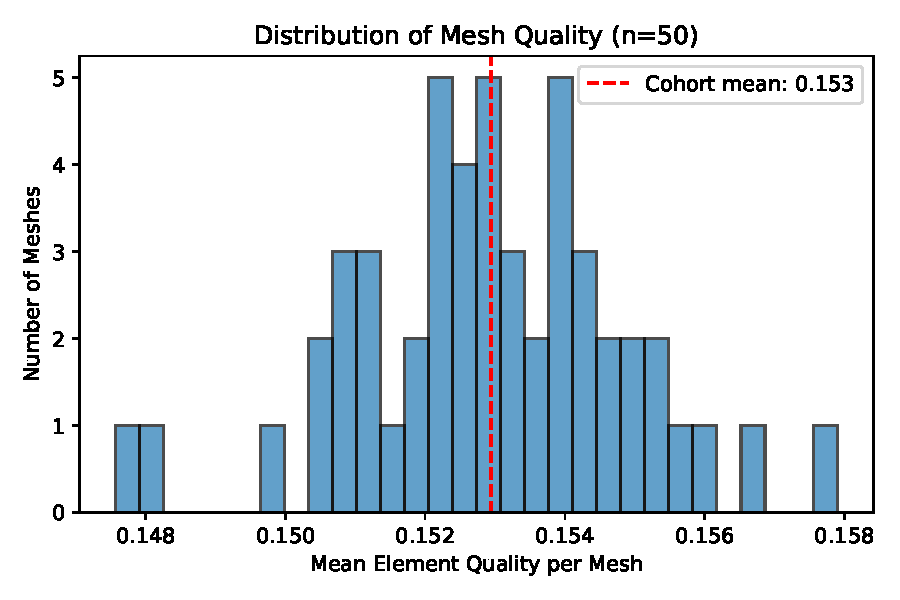
\includegraphics[width=0.8\textwidth]{S4_Fig}
    \caption{
        \textbf{Distribution of mean element quality across the 50-heart cohort.}
        Each point represents one mesh. The \texttt{tet\_qmetric\_volume} metric
        ranges from 0 (perfect tetrahedron) to 1 (degenerate); lower values
        indicate better quality. Cohort-wide mean was $0.153 \pm 0.100$.
        No inverted elements (quality $> 0.99$) were found in any mesh.
    }
    \label{fig:s4-mesh-quality-dist}
\end{figure}

\iffalse % Table replaced by Data file (supplementary/S*_Data_mesh_quality.csv); kept here for reference only.
\begin{landscape}
\begin{longtable}{lrcccccc}
\caption{
    \textbf{Per-model mesh quality statistics for all 50 hearts.}
    Quality metric: \texttt{tet\_qmetric\_volume} (0 = perfect tetrahedron,
    1 = fully degenerate). $N_{\text{el}}$: total element count
    ($\times 10^6$). Min/Max/Mean/SD: element quality statistics per mesh.
    $N_{\text{inv}}$: inverted elements (quality $> 0.99$).
    $N_{\text{deg}}$: near-degenerate elements (quality $> 0.90$).
} \\
\toprule
\textbf{Mesh ID} &
    $N_{\text{el}}$ ($\times 10^6$) &
    \textbf{Min} &
    \textbf{Max} &
    \textbf{Mean} &
    \textbf{SD} &
    $N_{\text{inv}}$ &
    $N_{\text{deg}}$ \\
\midrule
\endfirsthead
\multicolumn{8}{c}{\tablename\ \thetable{} (continued)} \\
\toprule
\textbf{Mesh ID} &
    $N_{\text{el}}$ ($\times 10^6$) &
    \textbf{Min} &
    \textbf{Max} &
    \textbf{Mean} &
    \textbf{SD} &
    $N_{\text{inv}}$ &
    $N_{\text{deg}}$ \\
\midrule
\endhead
\midrule
\multicolumn{8}{r}{\textit{Continued on next page}} \\
\endfoot
\bottomrule
\endlastfoot
3L9ZV4XS & 2.33 & $1.56\times10^{-4}$ & 0.926 & 0.157 & 0.102 & 0 & 2 \\
591DW86I  & 2.30 & $6.15\times10^{-5}$ & 0.845 & 0.153 & 0.100 & 0 & 0 \\
5IM7QJF4  & 2.26 & $1.25\times10^{-4}$ & 0.937 & 0.152 & 0.100 & 0 & 1 \\
627ZFI97  & 2.10 & $2.15\times10^{-4}$ & 0.874 & 0.156 & 0.101 & 0 & 0 \\
66AL590N  & 2.55 & $2.22\times10^{-4}$ & 0.901 & 0.152 & 0.100 & 0 & 1 \\
6G8DD8S5  & 2.82 & $2.64\times10^{-4}$ & 0.854 & 0.151 & 0.100 & 0 & 0 \\
7D98EVAR  & 2.41 & $1.94\times10^{-4}$ & 0.895 & 0.152 & 0.100 & 0 & 0 \\
98EK6960  & 2.29 & $1.13\times10^{-4}$ & 0.950 & 0.155 & 0.101 & 0 & 5 \\
98G5I5CE  & 3.08 & $1.02\times10^{-4}$ & 0.869 & 0.153 & 0.100 & 0 & 0 \\
9HE9S8YK  & 2.85 & $2.69\times10^{-4}$ & 0.910 & 0.154 & 0.100 & 0 & 2 \\
A1VMI1BL  & 2.52 & $3.21\times10^{-4}$ & 0.891 & 0.154 & 0.101 & 0 & 0 \\
A8NCPLRI  & 4.50 & $1.18\times10^{-4}$ & 0.890 & 0.153 & 0.100 & 0 & 0 \\
B782Q8ID  & 3.20 & $3.96\times10^{-5}$ & 0.978 & 0.151 & 0.099 & 0 & 4 \\
BJRXL8KY  & 2.74 & $1.94\times10^{-4}$ & 0.955 & 0.158 & 0.102 & 0 & 6 \\
BRUN0G9V  & 2.14 & $3.88\times10^{-4}$ & 0.972 & 0.155 & 0.101 & 0 & 3 \\
C21IDK9N  & 2.51 & $9.14\times10^{-5}$ & 0.918 & 0.153 & 0.100 & 0 & 1 \\
CTW6MAJL  & 1.88 & $2.86\times10^{-4}$ & 0.875 & 0.154 & 0.100 & 0 & 0 \\
D16RF7C3  & 1.98 & $2.44\times10^{-4}$ & 0.884 & 0.154 & 0.101 & 0 & 0 \\
DA8Q81SZ  & 2.95 & $1.92\times10^{-4}$ & 0.939 & 0.151 & 0.100 & 0 & 8 \\
DHIPF4L7  & 2.21 & $3.00\times10^{-4}$ & 0.905 & 0.154 & 0.100 & 0 & 1 \\
DN98C3EZ  & 2.09 & $2.57\times10^{-4}$ & 0.949 & 0.153 & 0.100 & 0 & 1 \\
FC14      & 3.12 & $7.25\times10^{-5}$ & 0.955 & 0.151 & 0.099 & 0 & 3 \\
FC15      & 2.23 & $1.83\times10^{-4}$ & 0.956 & 0.152 & 0.100 & 0 & 4 \\
FC5       & 1.99 & $3.12\times10^{-4}$ & 0.924 & 0.152 & 0.100 & 0 & 1 \\
FC7       & 2.14 & $9.35\times10^{-5}$ & 0.918 & 0.154 & 0.100 & 0 & 2 \\
FFI8S7CY  & 2.38 & $1.76\times10^{-4}$ & 0.845 & 0.151 & 0.100 & 0 & 0 \\
FM7ID9EE  & 2.46 & $4.11\times10^{-4}$ & 0.945 & 0.153 & 0.100 & 0 & 2 \\
FQB3LGOY  & 2.38 & $1.40\times10^{-4}$ & 0.935 & 0.153 & 0.100 & 0 & 2 \\
H2JQVUUF  & 1.90 & $4.51\times10^{-4}$ & 0.912 & 0.156 & 0.101 & 0 & 1 \\
LENYCA0B  & 3.30 & $1.40\times10^{-4}$ & 0.936 & 0.151 & 0.100 & 0 & 9 \\
LLWYK03H  & 2.04 & $1.88\times10^{-4}$ & 0.939 & 0.155 & 0.101 & 0 & 5 \\
MHFn31    & 2.97 & $3.79\times10^{-4}$ & 0.854 & 0.154 & 0.101 & 0 & 0 \\
MHFw14    & 3.33 & $2.32\times10^{-4}$ & 0.915 & 0.151 & 0.099 & 0 & 1 \\
MHFw16    & 2.67 & $4.34\times10^{-4}$ & 0.869 & 0.154 & 0.100 & 0 & 0 \\
MHFw6     & 3.49 & $4.72\times10^{-5}$ & 0.835 & 0.148 & 0.098 & 0 & 0 \\
MHFw8     & 3.18 & $1.67\times10^{-4}$ & 0.891 & 0.154 & 0.101 & 0 & 0 \\
MQWINMXL  & 3.43 & $2.31\times10^{-4}$ & 0.856 & 0.148 & 0.099 & 0 & 0 \\
N4TRHUUP  & 3.66 & $9.90\times10^{-5}$ & 0.964 & 0.151 & 0.100 & 0 & 5 \\
OA15VRI2  & 2.25 & $2.33\times10^{-4}$ & 0.850 & 0.153 & 0.100 & 0 & 0 \\
OHV835G6  & 2.01 & $2.26\times10^{-4}$ & 0.878 & 0.152 & 0.100 & 0 & 0 \\
PGXLUL41  & 3.41 & $2.38\times10^{-4}$ & 0.910 & 0.154 & 0.101 & 0 & 1 \\
PJR4AHZO  & 2.38 & $3.72\times10^{-4}$ & 0.925 & 0.151 & 0.099 & 0 & 1 \\
QSBZPFZI  & 2.11 & $1.65\times10^{-4}$ & 0.876 & 0.155 & 0.101 & 0 & 0 \\
SKSXRBWF  & 2.07 & $3.59\times10^{-4}$ & 0.912 & 0.155 & 0.101 & 0 & 1 \\
TCNI6BDU  & 2.48 & $1.76\times10^{-4}$ & 0.895 & 0.153 & 0.100 & 0 & 0 \\
TNJAF3TK  & 3.01 & $2.40\times10^{-4}$ & 0.895 & 0.152 & 0.100 & 0 & 0 \\
XBTL2UYF  & 2.77 & $2.45\times10^{-4}$ & 0.869 & 0.152 & 0.100 & 0 & 0 \\
XWSQF3JX  & 2.61 & $1.49\times10^{-4}$ & 0.882 & 0.155 & 0.101 & 0 & 0 \\
Y5HYEDL4  & 2.64 & $6.21\times10^{-5}$ & 0.908 & 0.153 & 0.100 & 0 & 1 \\
YCBD3S9F  & 4.33 & $5.34\times10^{-5}$ & 0.884 & 0.150 & 0.099 & 0 & 0 \\
Z8FT2XBQ  & 2.89 & $2.06\times10^{-4}$ & 0.871 & 0.153 & 0.100 & 0 & 0 \\
\end{longtable}
\end{landscape}
\fi

% --- end input:   sections/supp/s_fig4_mesh_quality ---


\nolinenumbers

\bibliography{myrefs}

\end{document}